% MIT License
%
% Copyright (c) 2022 Aliaksei Bialiauski
%
% Permission is hereby granted, free of charge, to any person obtaining a copy
% of this software and associated documentation files (the "Software"), to deal
% in the Software without restriction, including without limitation the rights
% to use, copy, modify, merge, publish, distribute, sublicense, and/or sell
% copies of the Software, and to permit persons to whom the Software is
% furnished to do so, subject to the following conditions:
%
% The above copyright notice and this permission notice shall be included in all
% copies or substantial portions of the Software.
%
% THE SOFTWARE IS PROVIDED "AS IS", WITHOUT WARRANTY OF ANY KIND, EXPRESS OR
% IMPLIED, INCLUDING BUT NOT LIMITED TO THE WARRANTIES OF MERCHANTABILITY,
% FITNESS FOR A PARTICULAR PURPOSE AND NONINFRINGEMENT. IN NO EVENT SHALL THE
% AUTHORS OR COPYRIGHT HOLDERS BE LIABLE FOR ANY CLAIM, DAMAGES OR OTHER
% LIABILITY, WHETHER IN AN ACTION OF CONTRACT, TORT OR OTHERWISE, ARISING FROM,
% OUT OF OR IN CONNECTION WITH THE SOFTWARE OR THE USE OR OTHER DEALINGS IN THE
% SOFTWARE.

\documentclass{article}
\usepackage{..//cover}
\usepackage{..//slides}
\usepackage{..//inno}
\usepackage[normalem]{ulem}
\newcommand*\thetitle{Management/}
\newcommand*\thesubtitle{MBO}
\begin{document}

    \plush{\defaultInnoTitlePage}

    \innoToc

    \plush{\innoChapter[MBO]{Management By Objectives}}

    \subcrumbection{Definition}
    \plush[4]{%
        \innoSection{Определение}
        \innoPic{0.6}{definition}
        \begin{itemize}
            \item MBO - подход в управлении организацией, когда руководство и сотрудники совместно определяют цели и планируют пути их достижения.
            \item сотрудники тоже вовлекаются в определение целей организации, выбор направления развития и принятия стратегических решений. MBO предполагает, что работа компании становится эффективнее, если все её сотрудники чётко понимают стоящие перед ними цели, знают, как оценивать свои результаты, и участвуют в обсуждении способов их достижения.
        \end{itemize}
    }

    \subcrumbection{SMART}
    \plush[4]{%
        \innoSection{SMART}
        \innoPic{0.6}{smart}
        Поставленные цели должны отвечать следующим условиям (для их запоминания используется мнемоническая аббревиатура SMART):
        \begin{itemize}
            \item S — specific «конкретные»;
            \item M — measurable «измеримые»;
            \item A — achievable «достижимые»;
            \item R — relevant «обоснованные»;
            \item T — time-based «ограниченные по времени».
            \item Traceable
            \item Verifiable
        \end{itemize}
    }

    \subcrumbection{MBO Flow}
    \plush{%
        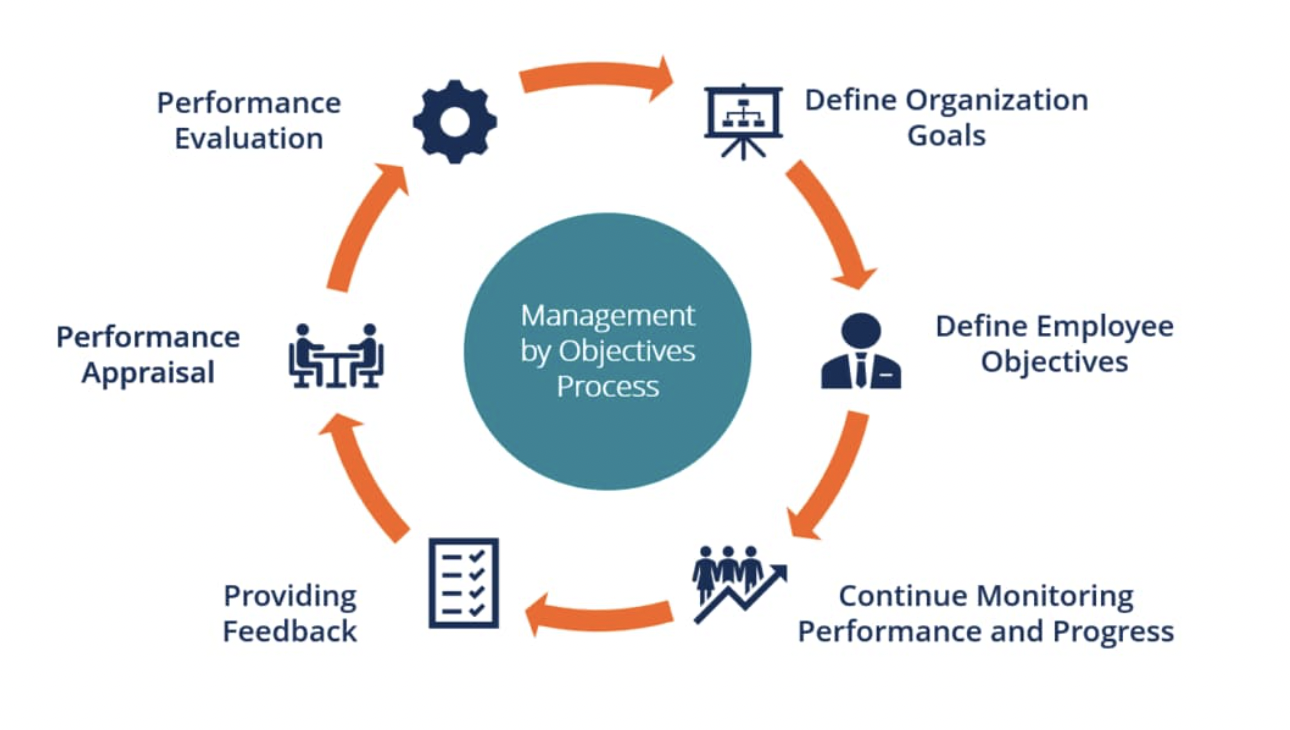
\includegraphics[scale=0.55]{..//images/books/mbo}
    }

    \subcrumbection{Pros and Cons}
    \plush[4]{%
        \innoSection{Плюсы и минусы MBO}
        \innoPic{0.6}{proscons}
        Плюсы:
        \begin{itemize}
            \item Детальное планирование, эстимация
            \item Более понятные роли и зона ответственности
        \end{itemize}
        Минусы:
        \begin{itemize}
            \item Проблемы с интеграцией процессов
            \item Нужны сильные менеджеры
        \end{itemize}
    }

    \plush{\innoChapter[OKR]{Objectives and Key Results}}

    \subcrumbection{OKR Components}
    \plush[6]{%
        \innoSection{Компоненты OKR}
        \innoPic{0.7}{okrcomponents}
        I will (Objective) as measured by (Key Results).
    }

    \subcrumbection{Objectives}
    \plush[6]{%
        \innoSection{Цели}
        \innoPic{0.6}{objectives}
        Цель — это просто то, что должно быть достигнуто, не больше и не меньше. По определению, цели значимы, конкретны, ориентированы на действия и (в идеале) вдохновляют. При правильном проектировании и применении они являются вакциной против нечеткого мышления и неэффективного исполнения.
    }

    \subcrumbection{Key Results}
    \plush[6]{%
        \innoSection{Результаты}
        \innoPic{0.7}{keyresults}
        Нужно оценивать и следить за тем, как мы достигаем цели. Эффективные KR являются конкретными, привязанными ко времени и агрессивными, но реалистичными. Прежде всего, они измеримы и проверяемы.
    }

    \plush{\innoChapter[SIMBA]{Simplified Management By Artifacts}}

    \subcrumbection{Why SIMBA?}
    \plush[3]{%
        \innoSection{Why SIMBA?}
        \innoPic{0.7}{whysimba}
        \begin{itemize}
            \item Нет мотивации, так как все получают зарплату за время, а не за результат
            \item Как следствие нет контроля над людьми, и соответственно результата
            \item MBO не работает!
        \end{itemize}
    }

    \subcrumbection{Plan}
    \plush[3]{%
        \innoSection{Plan}
        \innoPic{0.7}{plan}
        \begin{itemize}
            \item План - это документ, где каждая линия это артефакт
            \item Артефактом может быть что угодно
            \item За каждый артефакт ответственен \textbf{один} человек
        \end{itemize}
    }

    \subcrumbection{Learn SIMBA}
    \plush{%
        \innoQR{https://www.yegor256.com/2021/09/09/simba.html}
        Подробнее про SIMBA(автор - создатель методологии)
    }

    \plush{\innoBVC}

    \plush[4]{%
        \innoBanner{Call to Action:}
        \begin{itemize}
            \item Попробуйте делать личный план-менеджмент по SIMBA
            \item Попробуйте поставить несколько целей и продумать эстимацию по ним
            \item Попробуйте оценивать свои результаты каждый день и сравнивать их с предыдущими
        \end{itemize}
    }

    \plush[4]{%
        \innoBanner[orange]{Нерешенные вопросы:}
        \begin{itemize}
            \item Как определять цели и автоматически разбивать их на мелкие задачи?
            \item Как повысить качество в процессе выполнения целей?
            \item Как автоматически определять процент выполнения задач?
        \end{itemize}
    }

    \plush[4]{%
        \LARGE{Q\&A}
    }

\end{document}